\section{Modeling of Ablating Thermal Protection Systems}

This section presents the ablation problem for a non-decomposing TPS as a parametrized system of non-linear PDEs. These non-linear PDEs govern the energy of heat conduction and the pseudo-elastic material deformation of the mesh motion. Two different but mathematically-connected numerical solution strategies are provided: (1) a high-fidelity full-order model (FOM) based on a discontinuous Galerkin FEM, and (2) a thermo-elastic RPM based on a one-dimensional approximation to the energy and pseudo-elasticity equations.

\subsection{Governing Equations}\label{sec_governing_equations}

Consider a generic domain $\Omega\subset$, $d=2$ or $3$, illustrated in Fig.~\ref{fig_general_domain}. A heat flux $q_b(x,t)$ is prescribed on the boundary $\Gamma_q$ (i.e., Neumann boundary condition), and the temperature $T_b(x,t)$ is prescribed on boundary $\Gamma_T$ (i.e., Dirichlet boundary condition), where $\Gamma_q\cup\Gamma_T = \partial\Omega$ and $\Gamma_q\cap\Gamma_T = \emptyset$. The ablation occurs only on the heated boundary $\Gamma_q$, and its effects are included into the energy equation using an Arbitrary Lagrangian-Eulerian (ALE) description. The ALE assumes that the displacement $\vw(x,t)\in\mathbb{R}^d$ of the computational mesh moves with velocity $\vv(x,t)$ that is different to the material velocity, which is fixed to zero in this work.

\begin{figure}
    \centering
    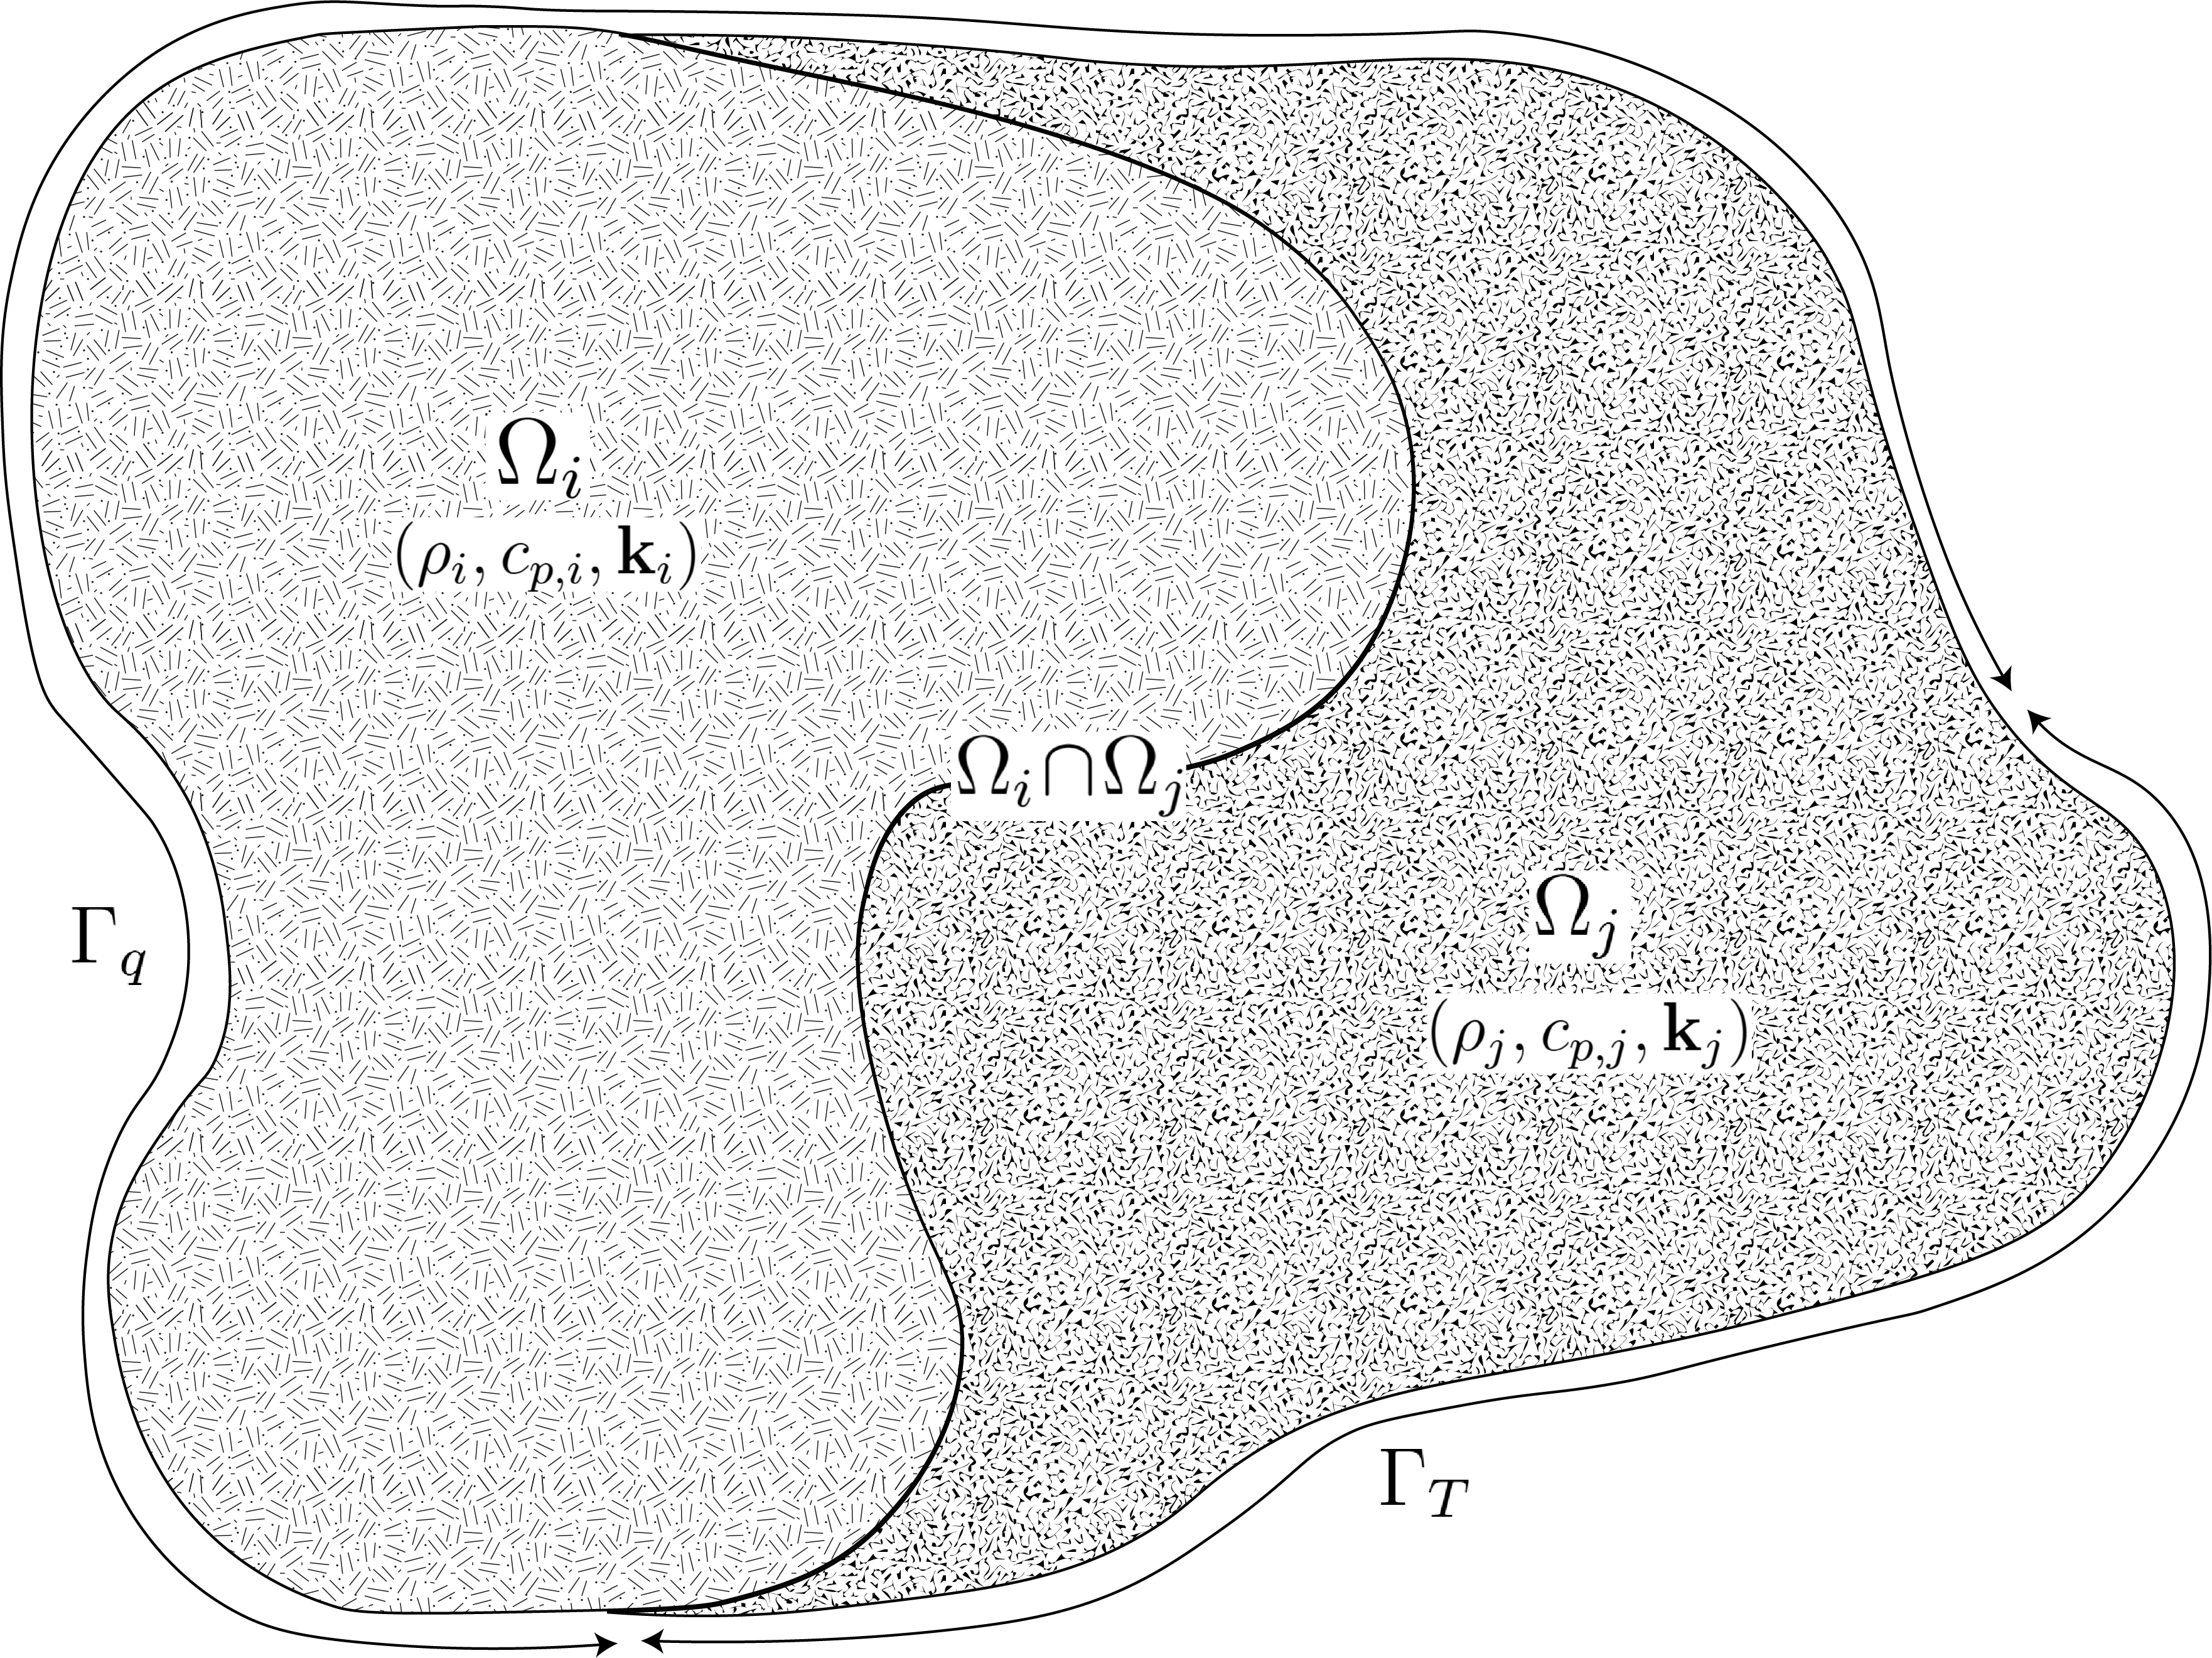
\includegraphics[width=0.6\textwidth]{./figs/general_domain.png}
    \caption{General domain $\Omega$ with prescribed heat flux $q_b(x,t)$ and temperature $T_b(x,t)$ on the boundaries $\Gamma_q$ and $\Gamma_T$, respectively. The mesh moves with a velocity $\mathbf{v}(x,t)$, while the material velocity is $\mathbf{w}(x,t)$.\hl{draw mesh next to arbitrary domain with moving boundaries.}}
    \label{fig_general_domain}
\end{figure}

The transient heat conduction is described by the energy equation,
\begin{subequations}
    \begin{align}
        \rho c_p\left(\ppt{T} - \mathbf{v}(x,t)\cdot\nabla T\right) - \nabla\cdot (\mathbf{k}\nabla T) &= \cQ(x,t),\ x\in\Omega \label{eqn_thermal_pde}\\
        -\mathbf{k}\nabla T\cdot \vn &= q_b(x,t),\ x\in\Gamma_q\label{eqn_thermal_bc_neumann}\\
        T(x,t) &= T_b(x,t),\ x\in\Gamma_T\label{eqn_thermal_bc_dirichlet}\\
        T(x,0) &= T_0(x),\ x\in\Omega\label{eqn_thermal_ic}
    \end{align}\label{eqn_governing_equations}
\end{subequations}
while the mesh motion is described by the pseudo-elasticity equation,
\begin{subequations}
    \begin{align}
        \nabla\cdot\boldsymbol{\sigma}(\mathbf{w}) &= 0\label{eqn_elasticity_pde}\\
        \vw(x,t) &= \vw_q(x,t),\quad x\in\Gamma_q\label{eqn_displacement_heated_bc}\\
        \vw(x,t) &= 0,\quad x\notin \Gamma_q\label{eqn_displacement_unheated_bc}\\
        \vw(x,0) &= \boldsymbol{0}\label{eqn_displacement_initial_condition}
    \end{align}
\end{subequations}

The density $\rho$, heat capacity $c_p$, and thermal conductivity $\mathbf{k}\in\mathbb{R}^{n_d\times n_d}$ are assumed to be constant with respect to temperature in this work. In the order they appear, the terms in \cref{eqn_thermal_pde} include, the unsteady energy storage, heat conduction, temperature advection due to mesh motion, and source terms due to boundary conditions.

The elasticity equation \cref{eqn_elasticity_pde} states that the divergence of the stress tensor $\boldsymbol{\sigma}(\mathbf{w})$ is zero. The stress tensor is related to the strain tensor $\bepsilon(\bw)$ through Hooke's law,
\[
    \boldsymbol{\sigma}(\bw) = \mathbb{D}:\boldsymbol{\epsilon}(\bw)
\]
where $\mathbb{D}$ is the constitutive operator, ``:'' is the double contraction of tensors, and $\bepsilon$ is the symmetric strain tensor given by,
\[
    \bepsilon(\bw) = \frac{1}{2}\left(\nabla\bw + \nabla\bw^T\right)
\]
For instance, an isotropic material assumption results in,
\[
    \bsigma = \lambda\left(\nabla\cdot\bw\right) \mathbf{I} + 2\mu\bepsilon(\bw)
\]
where $\lambda$ and $\mu$ are Lame constants that are arbitrarily selected to model the mesh motion. The ``material'' properties $\lambda$ and $\mu$ can be chosen to tailor the mesh deformation and need not represent the actual material being modeled~\hl{Amar2016}. 

The boundary conditions for the energy equation includes a heated surface (\cref{eqn_thermal_bc_neumann}) and a constant-temperature surface (\cref{eqn_thermal_bc_dirichlet}). The boundary conditions for the pseudo-elasticity equation are a function of the surface temperature $T_q(x,t)$ for $x\in\Gamma_q$ using a B' table. The B' table....
\begin{equation}
    \bw_q(x,t) = \int_{0}^{t} \mathbf{v}(x,\tau)d\tau = \int_{0}^{t}\mathbf{f}\left(T_q(x,\tau)\right)d\tau\label{eqn_boundary_displacement}
\end{equation}

\subsection{Full-Order Model: Finite-Element Method}\label{sec_fom}

Consider a conforming mesh partition domain, where each element belongs to one and only one component. Denote the collection of all $M$ elements as $\left\{E_i\right\}_{i=1}^{M}$. In an element $E_i$, its shared boundaries with another element $E_j$, Neumann BC, and Dirichlet BC are denoted as $e_{ij}$, $e_{iq}$, and $e_{iT}$, respectively. Lastly, $\left|e\right|$ denotes the length $(n_d=2)$ or area $(n_d=3)$ of a component boundary $e$.

For the $i$-th element, use a set of $P$ trial functions, such as polynomials, to represent the temperature distribution,
\begin{equation}
    T^{(i)}(x,t) = \sum_{l=1}^{P} \phi_l^{(i)}(x)u_l^{(i)} \equiv \boldsymbol{\phi}^{(i)}(x)^T\vu^{(i)}(t),\quad i=1,2,\dots,M\label{eqn_element_temperature}
\end{equation}
By standard variational processes, e.g., \hl{Cohen2018}, the element-wise governing equation is denoted as,
\begin{equation}
    \vA^{(i)}\dot{\vu}^{(i)} = \left(\vB^{(i)} + \vC^{(i)}(t)\right)\vui + \sumneighbordirichlet\left(\vB^{(i)}_{ij}\vui + \vB^{(j)}_{ij}\vuj\right) + \vf^{(i)}(t),\quad\text{for }i=1,2,\dots,M\label{eqn_element_dg}
\end{equation}
which is collected as the following ODE for the all the elements in the mesh,
\begin{equation}
    \vA(\vu)\dot{\vu} = \left[\vB(\vu) + \vC(t,\vu)\right]\vu + \mathbf{f}(t)\label{eqn_full_dg}
\end{equation}
where $\vu = \left[\vu^{(1)}, \vu^{(2)}, \ldots, \vu^{(M)}\right]^T\in\mathbb{R}^{MP}$ includes all the DG variables, $\mathbf{f}\in\mathbb{R}^{MP}$ is the external forcing, and the system matrices $\vA$, $\vB$, and $\vC$ are the matrices due to heat capacity, heat conduction, and temperature advection due to mesh motion, respectively. A detailed derivation of \cref{eqn_element_dg,eqn_full_dg} and their matrices is provided in Appendix~\hl{DG-FEM}.

\hl{need to discuss FOM for mesh displacement}

\subsection{Reduced-Physics Model: Lumped-Capacitance Model With Pseudo-Elastic Motion}


\subsubsection{Lumped Capacitance Model}
The main results for the lumped capacitance model (LCM) derivation are provided in this section and the mathematical details are provided in Appendix \hl{A}. The LCM is a classical physics-based low-order model for predicting the temporal variation of average temperature in multiple connected components \hl{INCROPERA}. The LCM is derived at the component level from a point of view of energy conservation, and leads to the following system of ODEs for the average temperatures on the components,
\begin{equation}
    \bar{\vA}\dot{\bar{\vu}} = \bar{\vB}\left(\bar{\vu}\right)\bar{\vu} + \bar{\vf}(t)\label{eqn_lcm}
\end{equation}
where,
\begin{subequations}
    \begin{align}
       \bar{\vu} &= \left[\bar{u}^{(1)},\bar{u}^{(2)},\dots,\bar{u}^{(N)}\right]^T\in\mathbb{R}^{N}\\
        \bar{\vf} &= \left[\bar{f}^{(1)},\bar{f}^{(2)},\dots,\bar{f}^{(N)}\right]^T\in\mathbb{R}^{N}
    \end{align}
\end{subequations}
includes the average temperatures $\bar{\vu}$ and forcing inputs $\bar{\vf}$ for the $N$ components. For $i,j=1,2,\dots,N$ the $(i,j)$-th elements of the $\bar{\vA}\in\mathbb{R}^{N\times N}$ and $\bar{\vB}\in\mathbb{R}^{N\times N}$ matrices are given by,
\begin{equation}
    \bar{A}^{(i)} = \begin{cases}
            \int_{\Omega^{(i)}}\rho c_p d\Omega^{(i)}, & i=j\\
            0, & i\neq j
        \end{cases},\quad \bar{B}_{ij} = \begin{cases}
        \sumneighbordirichlet\bar{B}^{(i)}_{ij}, &i=j \\
        \bar{B}^{(j)}_{ij}, & i\neq j
    \end{cases}
\end{equation}

\begin{figure}
    \centering
    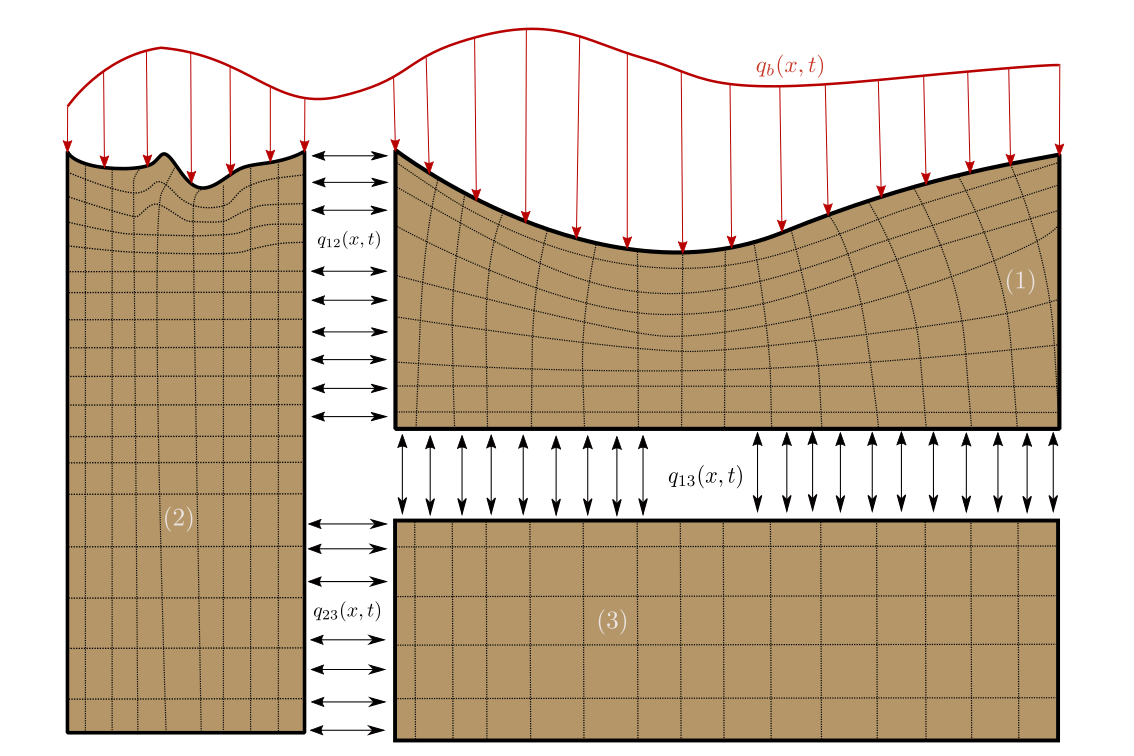
\includegraphics[width=0.8\textwidth]{./figs/three_components.png}
    \caption{Partition of the TPS into three layers.}
    \label{fig_lcm_domain}
\end{figure}

\subsubsection{Pseudo-Elastic Mesh Motion}

The components in the LCM are assumed to displace parallel to the direction of the applied heating, i.e., the $y$ direction in Fig.~\ref{fig_lcm_domain}. Therefore, the elasticity equation in \cref{eqn_elasticity_pde} for the $i$-th component simplifies to,
\begin{equation}
    \frac{\partial^2 w^{(i)}}{\partial x^2} = 0
\end{equation}
which has the analytical solution,
\begin{equation}
    w^{(i)}(y,t) = a(t)y + b(t)
\end{equation}
Imposing the boundary conditions leads to,
\begin{equation}
    w^{(i)}(x,t) = w^{(i)}(0,t)\left(\frac{y_1^{(i)} - y}{h^{(i)}}\right)
\end{equation}




Note that \cref{eqn_elasticity_1d} is steady. Under the assumption that the mesh deformation is quasi-steady, it can be applied at each time step within an ablation simulation. For instance, a known value of the wall temperature $T_w(t)$ specifies a Dirichlet boundary condition for the displacement, and the resulting nodal displacements within the ablator are determined from \cref{eqn_elasticity_pde}.

Along the one-dimensional domain, the PDE in \cref{eqn_elasticity_pde} simplifies to,
\begin{equation}
    \frac{\partial^2 u^{(i)}}{\partial x^2} = 0
\end{equation}
which has the analytical solution,
\begin{equation}
    u^{(i)}(x,t) = a(t)x + b(t)
\end{equation}
Imposing the boundary conditions leads to,
\begin{equation}
    u^{(i)}(x,t) = u^{(i)}(0,t)\left(\frac{x_1^{(i)} - x}{h^{(i)}}\right)
\end{equation}
The mesh velocity is the time derivative of the displacement,
\begin{equation}
    v^{(i)}(x,t) = \frac{\partial u^{(i)}(x,t)}{\partial t} = v^{(i)}(t)\left(\frac{x_1^{(i)} - x}{h^{(i)}}\right)
\end{equation}

\subsection{Summary of Modeling Approaches}

The FOM (i.e., DG-FEM) and RPM (i.e., LCM) are two different but mathematically connected solution startegies. Specifically, the LCM in \cref{eqn_lcm} not only resembles the functional form of the DG model in \cref{eqn_dg_fem}, but can be viewed as a special case of the latter, where the mesh partition is extremely coarse, and the trial and test functions are piece-wise constants. For example, consider the case where each component $\Omega^{(i)}$ is treated as one single element, and each element employs one constant basis function $\phi^{(i)}=1$. The element-wise DG model in \cref{eqn_element_dg} simplifies into a scalar ODE that ignores effects due to mesh motion,
\begin{equation}
    \vAi = \bar{A}^{(i)},\quad \vCi = 0, \quad\vBiij = -\sigma|\eij|,\quad \vBjij=\sigma|\eij|,\quad \vf^{(i)} = |\eiq|\bar{q}^{(i)} + \sigma|\eiT|\bar{T}^{(i)}
\end{equation}
Clearly, the LCM is a coarse zeroth-order DG model with the inverse of thermal resistance chosen as the element-wise penalty factors. Or conversely, the DG model is a refined version of LCM via \textit{hp}-adaptation.

On one hand, the FOM is the most accurate but computationally expensive to evaluate due to the fine mesh discretizations to possibly millions of state variables. On the other hand, the RPM considers only the average temperature of the material as the state variable, considerably reducing the computational cost, but sacrificing the fidelity of the temperature predictiona and neglecting higher-order effects due to mesh motion. Thus, neigher the FOM nor the RPM is a universal approach for real-world analysis, design, and optimization tasks for ablating TPS, where thounds of high-fidelity model evaluations may be necessary. This issue motivates the development of the PIROM, which can achieve the fidelity of FOM at a computational cost close to the RPM, while maintaining the generalizability to model parameters.



\subsubsection{Coupling Scheme}

\subsubsection{Reduced-Physics Ablation Simulation}







